\section*{Introduction}

How biology produces robust pattern in space and time is still largely an open question. Alan Turing proposed a mechanism but far from real biological complexity, and suffers from fine tuning, especially of diffusion parameters. And diffusion-driven instability is based on LSA…..Natural relevant phenomena such as growth, exotic boundary conditions, larger network size matter, and nonlinearities are often not addressed. A way forward is Feynman’s mantra using synthetic biology for small networks – connects to biology and industry applications, but Karig et al. and Selkine et al. (2018) stochastic not regular patterns, so question is largely unanswered. While Isalan lab can produce patterns (Fig. 1 – we have to ask him to include an image), they are highly variable so we need to know what might work. An “atlas” would help to guide experiments.

There has been considerable progress in terms of systematic studies of Turing patterns such as explorations on topology and network size [e.g. Haas & Goldstein (2021)], and atlas [Scholes et al. (2019)], but latter is based on LSA, Turing I only, and no growth so far from actual biology….

What’s known about growth, boundary conditions, nonlinear effects, pattern types/symmetries with nonlinear stability analysis [Ermentrout (1991); Nagorcka & Mooney (1992); Woolley, Krause, Gaffney (2021)], and alternative patterns (Hopf-Turing)…. Mathematical analysis often based on idealised domains, certain types of popular BCs, and artificial growth assumptions, e.g. linear or exponential with diluation [Madzvamuse et al. (2010)].

In this paper….here we combine atlas of all 2 and 3 node networks with growth, realistic boundary conditions for microbial colonies, and extend to other types of patterns (Hopf-Turing etc) and nonlinear effects (using numerics too). We find that switching of steady states, boundary induced patterns and … play an important role, and that…. This shows …(relevance in broader context).



% Place figure captions after the first paragraph in which they are cited.
\begin{figure}[!h]
    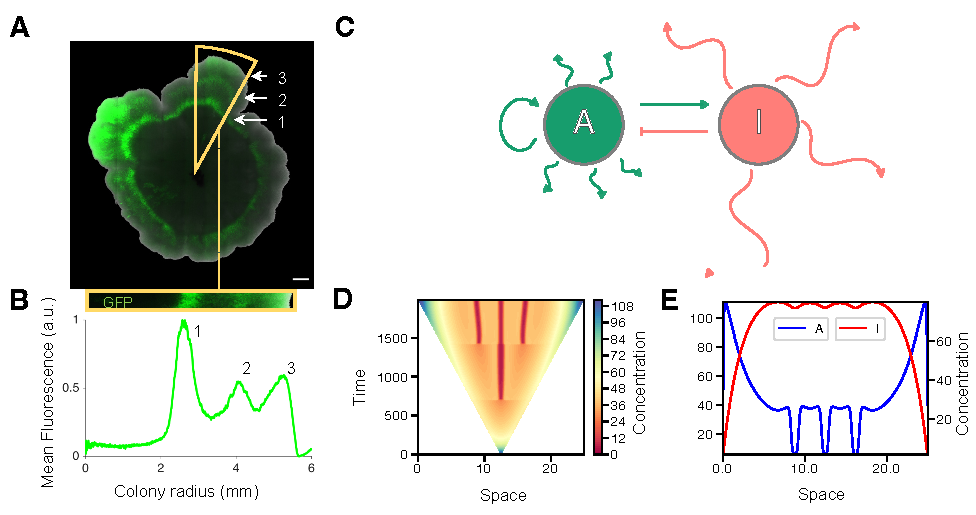
\includegraphics[width=1\textwidth]{figures/biological_example}

    \caption{{\bf Bold the figure title.}
        Figure caption text here, please use this space for the figure panel descriptions instead of using subfigure commands. A: Lorem ipsum dolor sit amet. B: Consectetur adipiscing elit.}
    \label{fig1}
\end{figure}
